%------------------------------------------------------------------------------
% Exemplo de documento para auxiliar a padronização das monografias da 
% Faculdade de Economia - UFF
%------------------------------------------------------------------------------

\documentclass[12pt, openright, chapter=TITLE]{economia} %---------------------
% Estão disponíveis opções de impressão como frente e verso, papel A4, outras
% linguagens e ets...
%------------------------------------------------------------------------------ 

%\usepackage{helvet}
%\renewcommand{\familydefault}{\sfdefault} % desmarcar as duas linhas de código para usar Arial como fonte...

\usepackage{pdfpages}

%------------------------------------------------------------------------------
% INFORMAÇÕES E DADOS PARA A CAPA
%------------------------------------------------------------------------------

\titulo{Aqui escrevemos o nome do Título: Modelo de Monografia em LaTeX  para a Faculdade de Economia UFF Niterói}
\autor{Gustavo de Oliveira Vital}
\data{2019} 
\orientador{Prof. Dr. Jesus Alexei Luizar Obregon}
\coorientador{Prof. Dr$^{a}$. Danielle Carusi Machado}


%------------------------------------------------------------------------------
%	FOLHA DE ROSTO E PREAMBULO
%------------------------------------------------------------------------------

\preambulo{Monografia apresentada ao curso de Bacharelado em Ciências Econômicas da Universidade Federal Fluminense como requisito parcial para conclusão do curso.}

%------------------------------------------------------------------------------
% INÍCIO DO DOCUMENTO
%------------------------------------------------------------------------------

\makeindex

\begin{document}

%------------------------------------------------------------------------------
% ELEMENTOS PRÉ-TEXTUAIS E CAPA
%------------------------------------------------------------------------------

%------------------------------------------------------------------------------
% Aqui iremos inserir, em ordem, a capa '\imprimircapa', a folha de rosto
% '\imprimirfolhaderosto*', as figuras da monografia '\figuras' e as tabelas
% 'tabelas'. É possível também a inserção de quadros, por exemplo, com o 
% comando 'quadros'. Sempre pulando uma linha entre as opções de ''listas''
%------------------------------------------------------------------------------

\imprimircapa 						
\imprimirfolhaderosto*	  					

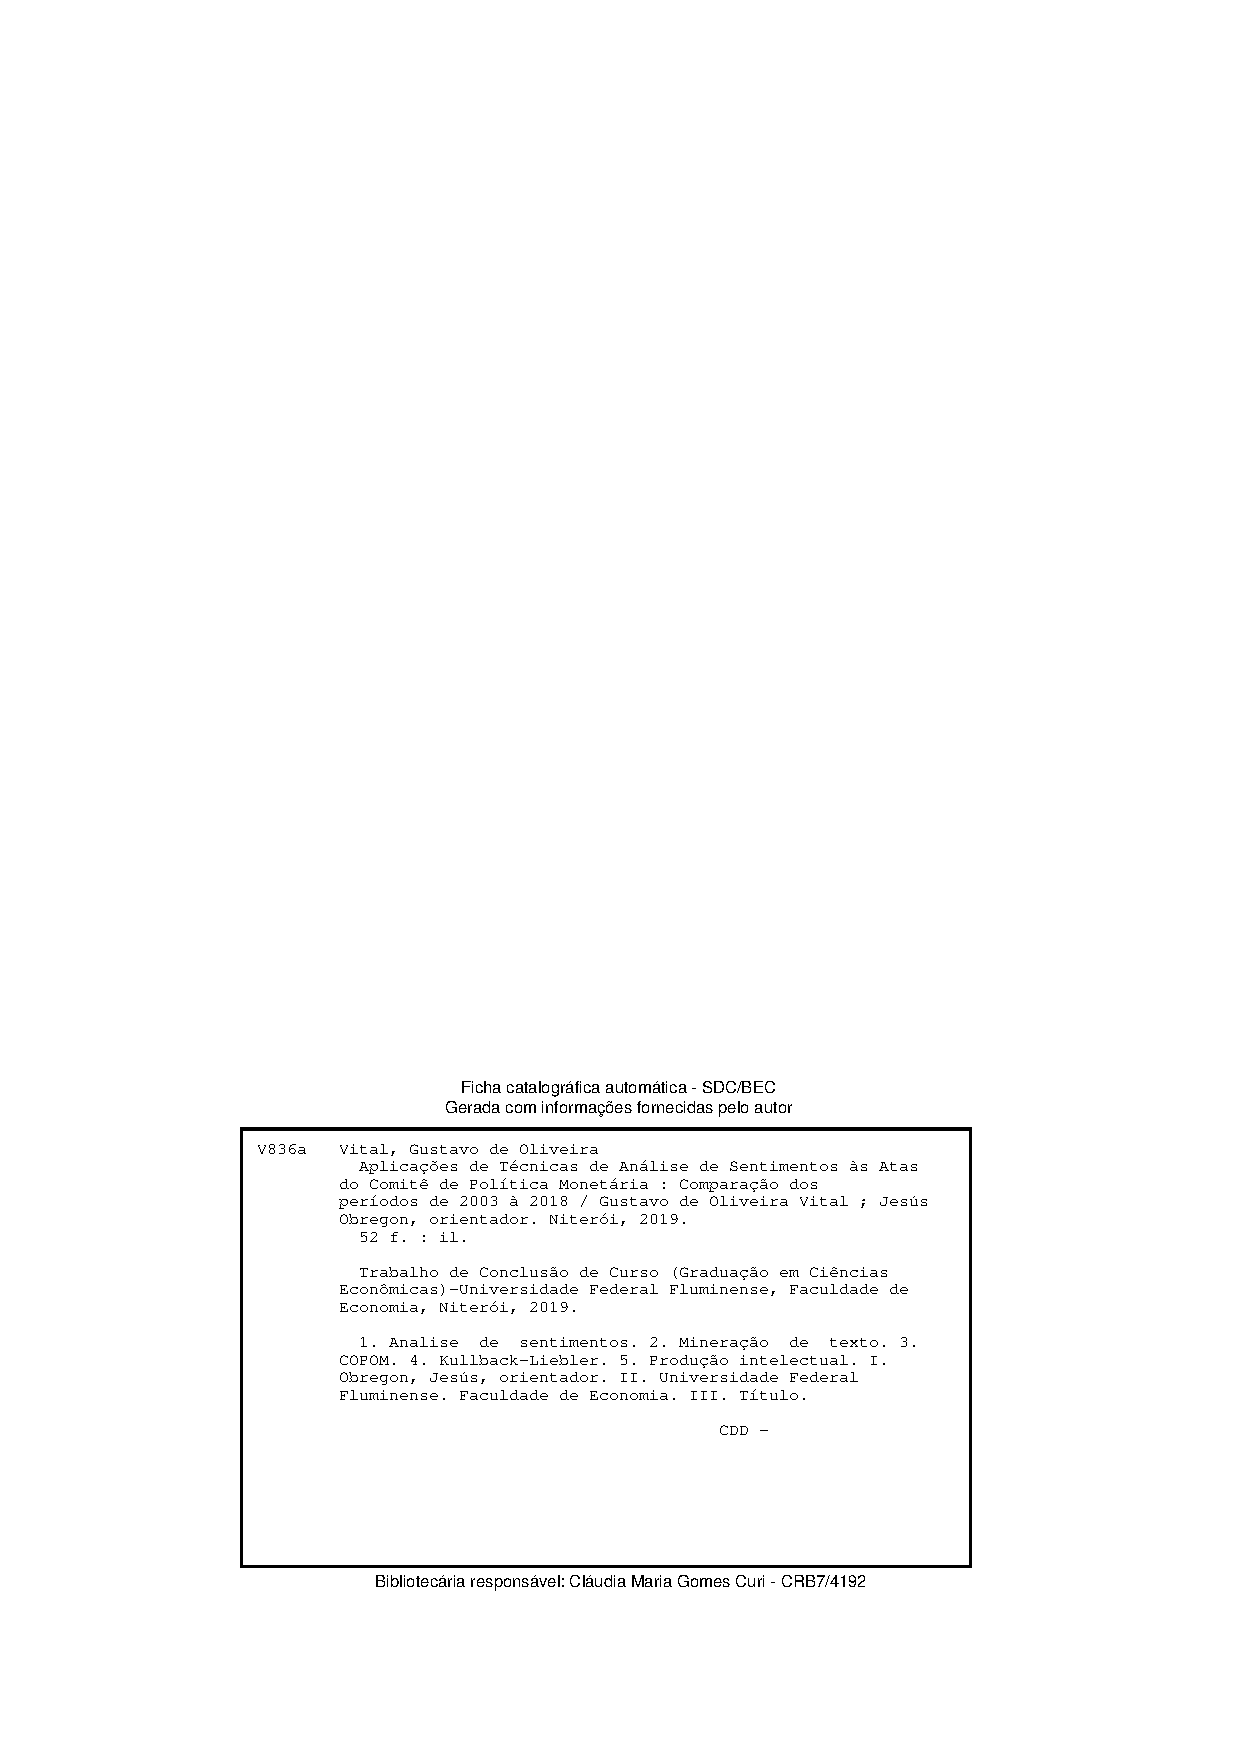
\includepdf[pages=1]{file.pdf} % inclui o arquivo file (ficha catalografica gerada pela biblioteca)
\begin{folhadeaprovacao}

   	\pre
   
   	\vfill
   	Trabalho aprovado em 21 de setembro de 2019\\
   	\banca
   	\assinatura{\textbf{\imprimirorientador}\space Orientador \\ \uff} 
   	\assinatura{\textbf{Professor} \\ \uff} % Escrever o nome do professor
   	\assinatura{\textbf{Professor} \\ \uff} % Se for outra instituição, escrever o nome
   	%\assinatura{\textbf{Professor} \\ Convidado 3}
   	%\assinatura{\textbf{Professor} \\ Convidado 4}
   	\vfill
	  
\end{folhadeaprovacao}	
\clearpage

% ------------------------------------------------------------------
% RESUMO E ABSTRACT
%
% Para iniciarmos um ambiente, seja de resumo, abstract ou outro 
% qualquer, devemos começar pelo \begin. Onde eu escrevo nesse 
% arquivo, já me encontro dentro de um ``ambiente de resumo''.
%
% Aqui, apresentarei o resumo e mais um outro comando de exemplo: o 
% \lipsum. A principal função do \lipsum é gerar textos aleatórios -
% textos dummys. Assim, por mais que no presente documento - 
% no arquivo .TeX - os \lipsum[3-5] ou \lipsum[2-4] apareçam, no 
% .pdf esses só aparecerão como textos aleatórios.
% ------------------------------------------------------------------

%\setlength{\absparsep}{18pt} % ajusta o espaçamento dos parágrafos do resumo
\begin{resumo}


	%-------------------------------------%
	%       AQUI ESCREVEMOS O TEXTO       %
	%-------------------------------------%
	

\lipsum[3-4] % GERAMOS UM TEXTO DUMMY

\textbf{Palavras-chave}: Latex; Abntex; Lipsum; Economia. % Palavra-chave inicia-se com maiúscula
\end{resumo}

% ------------------------------------------------------------------
% No caso do abstract, faremos a mesma coisa. Só adicionaremos a 
% opção abstract como o argumento do comando.
%-------------------------------------------------------------------

\begin{resumo}[ABSTRACT] % ESCREVER EM LETRAS MAIÚSCULAS
	
\lipsum[2-3] % Novamente o lipsum...

\textbf{Keywords}: Latex; Abntex; Lipsum; Economics. 	
\end{resumo}



	


\begin{dedicatoria}
	\vspace*{\fill}
	\centering
	\noindent
	\textit{ Este trabalho é dedicado às crianças adultas que,\\
		quando pequenas, sonharam em se tornar cientistas.} \vspace*{\fill}
\end{dedicatoria}
% ---

% ---
% Agradecimentos
% ---
\begin{agradecimentos}

	Agradeço primeiramente a esta universidade, seu corpo docente, direção e administração que proporcionaram a janela que hoje vislumbro um horizonte superior, eivado pela acendra confiança no mérito e ética aqui presentes. 
	
	Agradeço a todos os professores por me proporcionar o conhecimento não apenas racional, mas a manifestação do caráter e afetividade da educação no processo de formação profissional, por tanto que se dedicaram a mim não somente por terem ensinado, mas por terem me feito aprender.
	
	A palavra mestre, nunca fará justiça aos professores dedicados aos quais sem nominar terão meus eternos agradecimentos.

\end{agradecimentos}		
					
\figuras

\tabelas

\sumario


% -----------------------------------------------------------------------------
% ELEMENTOS TEXTUAIS
% -----------------------------------------------------------------------------

\textual



% ------------------------------------------------------------------
% Exemplo de introdução gerada por textos dummys a partir do
% lipsum
%-------------------------------------------------------------------


\chapter{Introdução}
Neste trabahlo querm

\label{cap:intro} % faço a referência na bibliografia

\lipsum[1]

%----------------------------------------------------------------------
\section{Motivação}
\label{sec:motivacao}
como escrevemos na parte (\ref{cap:intro})
\lipsum[2-4]

%----------------------------------------------------------------------
\subsection{Objetivos}
\label{sec:objetivos}

\lipsum[2-5]

%----------------------------------------------------------------------
\section{Estrutura do Trabalho}
\label{sec:estrutura}

\lipsum[1]

% ------------------------------------------------------------------
% Aqui, o objetivo é mostrar como colocar uma imagem ou um gráfico 
% na presente monografia. tudo que faremos é usar um ambiente 
% gráfico e assim, iremos o gerar. 
%-------------------------------------------------------------------

%-------------------------------------------------------------------
% Novamente, para preenchermos o documento, usaremos o lipsum
%-------------------------------------------------------------------

\chapter{graficos}
\label{cap:graf}

%\lipsum[37]
%-------------------------------------------------------------------
% O que faremos abaixo é incluir uma imagem (formato JPG, mas 
% poderia ser outro formato) no pdf. O argumento width=\textwidth 
% ajusta a largura da imagem a largura da página
%-------------------------------------------------------------------

\begin{figure}[h]
	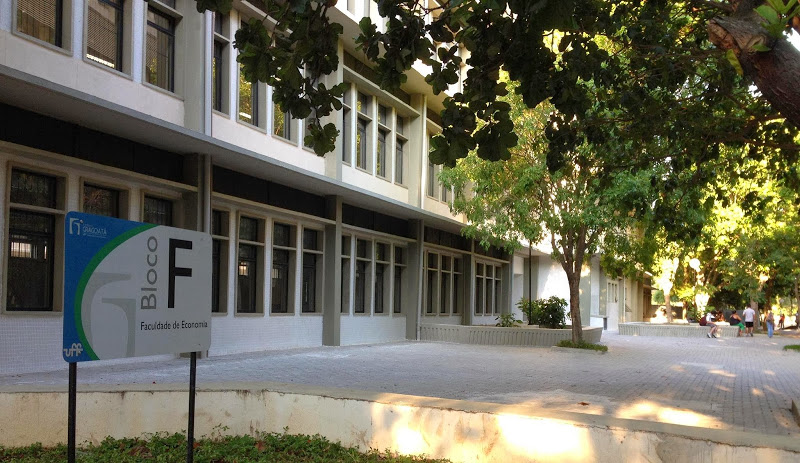
\includegraphics[width=\textwidth]{imagens/blocof.jpg}
	\caption{O Bloco F}
	\label{fig:blocof} % Aqui 'nomeamos' o gráfico
\end{figure}
A figura (\ref{fig:blocof})
%-------------------------------------------------------------------
% mais lipsum...
%-------------------------------------------------------------------

\lipsum[35-36]

% ------------------------------------------------------------------
% Aqui, o objetivo é mostrar como colocar uma tabela. Recomenda-se,
% quando necessário, a consulta no seguinte site:
%
%                https://www.tablesgenerator.com/
%
% Em que é possível criar suas próprias tabelas na mão, ou mesmo 
% importar do excel, por exemplo..
%-------------------------------------------------------------------

\chapter{tabelas}
\label{cap:tabelas}

%-------------------------------------------------------------------
% O que faremos abaixo é incluir uma tabela num ambiente table:
%-------------------------------------------------------------------

Criaremos uma tabela simples utilizando o ambiente tabular. Com o ambiente center, iremos centralizar:



\begin{table}[!h]
\centering
\begin{tabular}{lllll}
\hline
x & r & y & jk & d \\ \hline
1 & 2 & 3 & 3  & 1
\end{tabular}
\end{table}

Obviamente, podemos criar tabelas maiores e mais robustas. Nosso objetivo aqui, entretanto, não é esse. Que fique claro que outras \textit{N} possibilidades estão disponíveis. Segue um outro exemplo, feito diretamente utilizando a linguagem R:

\begin{table}[!htbp] \centering 
	\caption{Ajustes nos parâmetros} 
	\label{} 
	\begin{tabular}{@{\extracolsep{5pt}}lccc} 
		\\[-1.8ex]\hline 
		\hline \\[-1.8ex] 
								& \multicolumn{3}{c}{\textit{Dependent variable:}} \\ 
		\cline{2-4} 
		\\[-1.8ex] 				& \multicolumn{2}{c}{Overall Rating} 	& High Rating \\ 
		\\[-1.8ex] 				& \multicolumn{2}{c}{\textit{OLS}} 		& \textit{probit} \\ 
		\\[-1.8ex]				& (1) 			& (2) 					& (3)\\ 
		\hline \\[-1.8ex] 
		Handling of Complaints 	& 0.692$^{***}$ & 0.682$^{***}$ 		&  \\ 
								& (0.149) 		& (0.129) 				&  \\ 
		No Special Privileges 	& $-$0.104 		& $-$0.103 				&  \\ 
								& (0.135) 		& (0.129) 				&  \\ 
		Opportunity to Learn 	& 0.249 		& 0.238$^{*}$ 			& 0.164$^{***}$ \\ 
								& (0.160) 		& (0.139) 				& (0.053) \\ 
		Performance-Based Raises& $-$0.033 		& 						&  \\ 
								& (0.202) 		&  						&  \\ 
		Too Critical			& 0.015 		&  						& $-$0.001 \\ 
								& (0.147)		&  						& (0.044) \\ 
		Advancement 			&  				&  						& $-$0.062 \\ 
								&  				&  						& (0.042) \\ 
		Constant 				& 11.011 		& 11.258 				& $-$7.476$^{**}$ \\ 
								& (11.704) 		& (7.318) 				& (3.570) \\ 
		\hline \\[-1.8ex] 
		Observations 			& 30 			& 30 					& 30 \\ 
		R$^{2}$ 				& 0.715			& 0.715 				&  \\ 
		Adjusted R$^{2}$ 		& 0.656 		& 0.682 				&  \\ 
		Akaike Inf. Crit. 		& 				&  						& 26.175 \\ 
		\hline 
		\hline \\[-1.8ex] 
		\textit{Note:}  		& \multicolumn{3}{r}{$^{*}$p$<$0.1; $^{**}$p$<$0.05; $^{***}$p$<$0.01} \\ 
	\end{tabular} 
	\label{table:2}
\end{table} 


%-------------------------------------------------------------------
% mais lipsum...
%-------------------------------------------------------------------

\lipsum[2-4]


%-------------------------------------------------------------------
% Aqui mostraremos, por fim, como realizar uma citação
%-------------------------------------------------------------------

\chapter{Como Citar}
\label{cap:cite}

Supondo que desejássemos realizar uma citação no texto, por exemplo do pacote que usamos para fazer esse modelo de monografia. Tudo que teríamos que fazer seria utilizar o comando \texttt{citeonline\{\}} ou o \texttt{cite\{\}}. Usando o ambiente de citação, teríamos abaixo o exemplo.\cite{osbourne2009ozzy}

\begin{citacao}
	``Exemplo de um ambiente de citação. Não usamos o comando \texttt{citeonline\{\}}. Então, ao fim do ambiente iremos usar, entre parênteses para simular uma citação em ABNT.'' \cite[p.56]{osbourne2009ozzy}
\end{citacao}

aqui é um exemplo \citeonline{shapiro1997real}


\chapter{Conclusões}
\label{cap:conclusoes}

Vimos, então, que podemos escrever sem muitas dificuldades uma monografia em padrão ABNT sem nos preocuparmos a fundo com a padronização do documento, visto que o \LaTeX nos proporciona a confiabilidade necessária para uma automática padronização.

Indubitavelmente, desta forma, além de pouparmos tempos com regras e rigor podemos ainda manter um documento padrão para a Faculdade de Economia da Universidade Federal Fluminense.

Vimos como inserir tabelas, imagens, sumário e organizar um exemplo de monografia, com esse próprio exemplo de monografia. Por fim, vale ressaltar que o \LaTeX vai \textbf{muito além} deste documento, e suas próprias possibilidades dentro da classe \abnTeX\space ou mesmo da classe \texttt{economia} são infinitas. Assim, é extremamente válido uma busca mais a fundo para pontos de dúvidas. 

A primeira versão desse documento/classe foi concluída no dia 22/04/2019. Pretende-se, entretanto, manter essa classe em desenvolvimento quando necessário bem como em evolução. \textbf{qualquer} dúvida/sugestão, pode ser enviada para \textbf{\texttt{gustavovital@id.uff.br}}. O interesse em colaborar, também é bastante bem vindo e válido.




% ----------------------------------------------------------
% ELEMENTOS PÓS-TEXTUAIS
% ----------------------------------------------------------
\postextual

% ----------------------------------------------------------
% Referências bibliográficas
% ----------------------------------------------------------

\nocite{hobsbawm1995era,
		battista2000reduction,
		abntexmanual, 
		abntex2modelo} % aqui citamos os autores que não foram citados no texto.

\bibliography{referencias}


\end{document}
